\documentclass[twoside]{book}

% Packages required by doxygen
\usepackage{calc}
\usepackage{doxygen}
\usepackage{graphicx}
\usepackage[utf8]{inputenc}
\usepackage{makeidx}
\usepackage{multicol}
\usepackage{multirow}
\usepackage{textcomp}
\usepackage[table]{xcolor}

% Font selection
\usepackage[T1]{fontenc}
\usepackage{mathptmx}
\usepackage[scaled=.90]{helvet}
\usepackage{courier}
\usepackage{amssymb}
\usepackage{sectsty}
\renewcommand{\familydefault}{\sfdefault}
\allsectionsfont{%
  \fontseries{bc}\selectfont%
  \color{darkgray}%
}
\renewcommand{\DoxyLabelFont}{%
  \fontseries{bc}\selectfont%
  \color{darkgray}%
}

% Page & text layout
\usepackage{geometry}
\geometry{%
  a4paper,%
  top=2.5cm,%
  bottom=2.5cm,%
  left=2.5cm,%
  right=2.5cm%
}
\tolerance=750
\hfuzz=15pt
\hbadness=750
\setlength{\emergencystretch}{15pt}
\setlength{\parindent}{0cm}
\setlength{\parskip}{0.2cm}
\makeatletter
\renewcommand{\paragraph}{%
  \@startsection{paragraph}{4}{0ex}{-1.0ex}{1.0ex}{%
    \normalfont\normalsize\bfseries\SS@parafont%
  }%
}
\renewcommand{\subparagraph}{%
  \@startsection{subparagraph}{5}{0ex}{-1.0ex}{1.0ex}{%
    \normalfont\normalsize\bfseries\SS@subparafont%
  }%
}
\makeatother

% Headers & footers
\usepackage{fancyhdr}
\pagestyle{fancyplain}
\fancyhead[LE]{\fancyplain{}{\bfseries\thepage}}
\fancyhead[CE]{\fancyplain{}{}}
\fancyhead[RE]{\fancyplain{}{\bfseries\leftmark}}
\fancyhead[LO]{\fancyplain{}{\bfseries\rightmark}}
\fancyhead[CO]{\fancyplain{}{}}
\fancyhead[RO]{\fancyplain{}{\bfseries\thepage}}
\fancyfoot[LE]{\fancyplain{}{}}
\fancyfoot[CE]{\fancyplain{}{}}
\fancyfoot[RE]{\fancyplain{}{\bfseries\scriptsize Generated on Sun Jul 27 2014 00\-:18\-:38 for Network traffic simulator by Doxygen }}
\fancyfoot[LO]{\fancyplain{}{\bfseries\scriptsize Generated on Sun Jul 27 2014 00\-:18\-:38 for Network traffic simulator by Doxygen }}
\fancyfoot[CO]{\fancyplain{}{}}
\fancyfoot[RO]{\fancyplain{}{}}
\renewcommand{\footrulewidth}{0.4pt}
\renewcommand{\chaptermark}[1]{%
  \markboth{#1}{}%
}
\renewcommand{\sectionmark}[1]{%
  \markright{\thesection\ #1}%
}

% Indices & bibliography
\usepackage{natbib}
\usepackage[titles]{tocloft}
\setcounter{tocdepth}{3}
\setcounter{secnumdepth}{5}
\makeindex

% Hyperlinks (required, but should be loaded last)
\usepackage{ifpdf}
\ifpdf
  \usepackage[pdftex,pagebackref=true]{hyperref}
\else
  \usepackage[ps2pdf,pagebackref=true]{hyperref}
\fi
\hypersetup{%
  colorlinks=true,%
  linkcolor=blue,%
  citecolor=blue,%
  unicode%
}

% Custom commands
\newcommand{\clearemptydoublepage}{%
  \newpage{\pagestyle{empty}\cleardoublepage}%
}


%===== C O N T E N T S =====

\begin{document}

% Titlepage & ToC
\hypersetup{pageanchor=false}
\pagenumbering{roman}
\begin{titlepage}
\vspace*{7cm}
\begin{center}%
{\Large Network traffic simulator \\[1ex]\large 1.\-0 }\\
\vspace*{1cm}
{\large Generated by Doxygen 1.8.6}\\
\vspace*{0.5cm}
{\small Sun Jul 27 2014 00:18:38}\\
\end{center}
\end{titlepage}
\clearemptydoublepage
\tableofcontents
\clearemptydoublepage
\pagenumbering{arabic}
\hypersetup{pageanchor=true}

%--- Begin generated contents ---
\chapter{Namespace Index}
\section{Namespace List}
Here is a list of all namespaces with brief descriptions\-:\begin{DoxyCompactList}
\item\contentsline{section}{\hyperlink{namespaceMFF__NPRG031}{M\-F\-F\-\_\-\-N\-P\-R\-G031} }{\pageref{namespaceMFF__NPRG031}}{}
\item\contentsline{section}{\hyperlink{namespaceNetTrafficSimulator}{Net\-Traffic\-Simulator} }{\pageref{namespaceNetTrafficSimulator}}{}
\item\contentsline{section}{\hyperlink{namespaceStetic}{Stetic} }{\pageref{namespaceStetic}}{}
\end{DoxyCompactList}

\chapter{Hierarchical Index}
\section{Class Hierarchy}
This inheritance list is sorted roughly, but not completely, alphabetically\-:\begin{DoxyCompactList}
\item \contentsline{section}{M\-F\-F\-\_\-\-N\-P\-R\-G031.\-Calendar}{\pageref{classMFF__NPRG031_1_1Calendar}}{}
\item \contentsline{section}{Net\-Traffic\-Simulator.\-Link.\-Data\-Envelope}{\pageref{classNetTrafficSimulator_1_1Link_1_1DataEnvelope}}{}
\item \contentsline{section}{M\-F\-F\-\_\-\-N\-P\-R\-G031.\-Event}{\pageref{classMFF__NPRG031_1_1Event}}{}
\item \contentsline{section}{Net\-Traffic\-Simulator.\-I\-Addressable}{\pageref{interfaceNetTrafficSimulator_1_1IAddressable}}{}
\begin{DoxyCompactList}
\item \contentsline{section}{Net\-Traffic\-Simulator.\-End\-Node}{\pageref{classNetTrafficSimulator_1_1EndNode}}{}
\item \contentsline{section}{Net\-Traffic\-Simulator.\-Server\-Node}{\pageref{classNetTrafficSimulator_1_1ServerNode}}{}
\end{DoxyCompactList}
\item \contentsline{section}{Net\-Traffic\-Simulator.\-I\-Namable}{\pageref{interfaceNetTrafficSimulator_1_1INamable}}{}
\begin{DoxyCompactList}
\item \contentsline{section}{Net\-Traffic\-Simulator.\-Link}{\pageref{classNetTrafficSimulator_1_1Link}}{}
\item \contentsline{section}{Net\-Traffic\-Simulator.\-Node}{\pageref{classNetTrafficSimulator_1_1Node}}{}
\begin{DoxyCompactList}
\item \contentsline{section}{Net\-Traffic\-Simulator.\-End\-Node}{\pageref{classNetTrafficSimulator_1_1EndNode}}{}
\item \contentsline{section}{Net\-Traffic\-Simulator.\-Network\-Node}{\pageref{classNetTrafficSimulator_1_1NetworkNode}}{}
\item \contentsline{section}{Net\-Traffic\-Simulator.\-Server\-Node}{\pageref{classNetTrafficSimulator_1_1ServerNode}}{}
\end{DoxyCompactList}
\end{DoxyCompactList}
\item \contentsline{section}{Net\-Traffic\-Simulator.\-I\-Result\-Provider}{\pageref{interfaceNetTrafficSimulator_1_1IResultProvider}}{}
\begin{DoxyCompactList}
\item \contentsline{section}{Net\-Traffic\-Simulator.\-End\-Node}{\pageref{classNetTrafficSimulator_1_1EndNode}}{}
\item \contentsline{section}{Net\-Traffic\-Simulator.\-Link}{\pageref{classNetTrafficSimulator_1_1Link}}{}
\item \contentsline{section}{Net\-Traffic\-Simulator.\-Network\-Node}{\pageref{classNetTrafficSimulator_1_1NetworkNode}}{}
\item \contentsline{section}{Net\-Traffic\-Simulator.\-Server\-Node}{\pageref{classNetTrafficSimulator_1_1ServerNode}}{}
\end{DoxyCompactList}
\item \contentsline{section}{Net\-Traffic\-Simulator.\-Main\-Class}{\pageref{classNetTrafficSimulator_1_1MainClass}}{}
\item \contentsline{section}{M\-F\-F\-\_\-\-N\-P\-R\-G031.\-Model}{\pageref{classMFF__NPRG031_1_1Model}}{}
\item \contentsline{section}{Net\-Traffic\-Simulator.\-Network\-Model}{\pageref{classNetTrafficSimulator_1_1NetworkModel}}{}
\item \contentsline{section}{Net\-Traffic\-Simulator.\-Network\-Model\-Test}{\pageref{classNetTrafficSimulator_1_1NetworkModelTest}}{}
\item \contentsline{section}{Net\-Traffic\-Simulator.\-Packet}{\pageref{classNetTrafficSimulator_1_1Packet}}{}
\item \contentsline{section}{M\-F\-F\-\_\-\-N\-P\-R\-G031.\-Process}{\pageref{classMFF__NPRG031_1_1Process}}{}
\begin{DoxyCompactList}
\item \contentsline{section}{Net\-Traffic\-Simulator.\-Link}{\pageref{classNetTrafficSimulator_1_1Link}}{}
\item \contentsline{section}{Net\-Traffic\-Simulator.\-Node}{\pageref{classNetTrafficSimulator_1_1Node}}{}
\end{DoxyCompactList}
\item \contentsline{section}{Net\-Traffic\-Simulator.\-Result\-Model}{\pageref{classNetTrafficSimulator_1_1ResultModel}}{}
\item \contentsline{section}{Net\-Traffic\-Simulator.\-Simulation\-Controller}{\pageref{classNetTrafficSimulator_1_1SimulationController}}{}
\item \contentsline{section}{Net\-Traffic\-Simulator.\-Simulation\-Controller\-Test}{\pageref{classNetTrafficSimulator_1_1SimulationControllerTest}}{}
\item \contentsline{section}{Net\-Traffic\-Simulator.\-Simulation\-Model}{\pageref{classNetTrafficSimulator_1_1SimulationModel}}{}
\item \contentsline{section}{Net\-Traffic\-Simulator.\-Simulation\-Model\-Test}{\pageref{classNetTrafficSimulator_1_1SimulationModelTest}}{}
\item \contentsline{section}{M\-F\-F\-\_\-\-N\-P\-R\-G031.\-State}{\pageref{classMFF__NPRG031_1_1State}}{}
\item Window\begin{DoxyCompactList}
\item \contentsline{section}{Main\-Window}{\pageref{classMainWindow}}{}
\end{DoxyCompactList}
\end{DoxyCompactList}

\chapter{Class Index}
\section{Class List}
Here are the classes, structs, unions and interfaces with brief descriptions\-:\begin{DoxyCompactList}
\item\contentsline{section}{\hyperlink{classNetTrafficSimulator_1_1MainClass}{Net\-Traffic\-Simulator.\-Main\-Class} }{\pageref{classNetTrafficSimulator_1_1MainClass}}{}
\item\contentsline{section}{\hyperlink{classMainWindow}{Main\-Window} }{\pageref{classMainWindow}}{}
\item\contentsline{section}{\hyperlink{classNetTrafficSimulator_1_1NetworkModel}{Net\-Traffic\-Simulator.\-Network\-Model} }{\pageref{classNetTrafficSimulator_1_1NetworkModel}}{}
\item\contentsline{section}{\hyperlink{classNetTrafficSimulator_1_1NetworkModelTest}{Net\-Traffic\-Simulator.\-Network\-Model\-Test} }{\pageref{classNetTrafficSimulator_1_1NetworkModelTest}}{}
\end{DoxyCompactList}

\chapter{File Index}
\section{File List}
Here is a list of all files with brief descriptions\-:\begin{DoxyCompactList}
\item\contentsline{section}{Net\-Traffic\-Simulator/\-Net\-Traffic\-Simulator/\hyperlink{MainWindow_8cs}{Main\-Window.\-cs} }{\pageref{MainWindow_8cs}}{}
\item\contentsline{section}{Net\-Traffic\-Simulator/\-Net\-Traffic\-Simulator/\hyperlink{Program_8cs}{Program.\-cs} }{\pageref{Program_8cs}}{}
\item\contentsline{section}{Net\-Traffic\-Simulator/\-Net\-Traffic\-Simulator/controller/\hyperlink{SimulationController_8cs}{Simulation\-Controller.\-cs} }{\pageref{SimulationController_8cs}}{}
\item\contentsline{section}{Net\-Traffic\-Simulator/\-Net\-Traffic\-Simulator/controller/\hyperlink{SimulationControllerTest_8cs}{Simulation\-Controller\-Test.\-cs} }{\pageref{SimulationControllerTest_8cs}}{}
\item\contentsline{section}{Net\-Traffic\-Simulator/\-Net\-Traffic\-Simulator/framework/\hyperlink{Calendar_8cs}{Calendar.\-cs} }{\pageref{Calendar_8cs}}{}
\item\contentsline{section}{Net\-Traffic\-Simulator/\-Net\-Traffic\-Simulator/framework/\hyperlink{Event_8cs}{Event.\-cs} }{\pageref{Event_8cs}}{}
\item\contentsline{section}{Net\-Traffic\-Simulator/\-Net\-Traffic\-Simulator/framework/\hyperlink{Model_8cs}{Model.\-cs} }{\pageref{Model_8cs}}{}
\item\contentsline{section}{Net\-Traffic\-Simulator/\-Net\-Traffic\-Simulator/framework/\hyperlink{Process_8cs}{Process.\-cs} }{\pageref{Process_8cs}}{}
\item\contentsline{section}{Net\-Traffic\-Simulator/\-Net\-Traffic\-Simulator/framework/\hyperlink{State_8cs}{State.\-cs} }{\pageref{State_8cs}}{}
\item\contentsline{section}{Net\-Traffic\-Simulator/\-Net\-Traffic\-Simulator/framework/extension/\hyperlink{EndNode_8cs}{End\-Node.\-cs} }{\pageref{EndNode_8cs}}{}
\item\contentsline{section}{Net\-Traffic\-Simulator/\-Net\-Traffic\-Simulator/framework/extension/\hyperlink{Link_8cs}{Link.\-cs} }{\pageref{Link_8cs}}{}
\item\contentsline{section}{Net\-Traffic\-Simulator/\-Net\-Traffic\-Simulator/framework/extension/\hyperlink{NetworkNode_8cs}{Network\-Node.\-cs} }{\pageref{NetworkNode_8cs}}{}
\item\contentsline{section}{Net\-Traffic\-Simulator/\-Net\-Traffic\-Simulator/framework/extension/\hyperlink{Node_8cs}{Node.\-cs} }{\pageref{Node_8cs}}{}
\item\contentsline{section}{Net\-Traffic\-Simulator/\-Net\-Traffic\-Simulator/framework/extension/\hyperlink{Packet_8cs}{Packet.\-cs} }{\pageref{Packet_8cs}}{}
\item\contentsline{section}{Net\-Traffic\-Simulator/\-Net\-Traffic\-Simulator/framework/extension/\hyperlink{ServerNode_8cs}{Server\-Node.\-cs} }{\pageref{ServerNode_8cs}}{}
\item\contentsline{section}{Net\-Traffic\-Simulator/\-Net\-Traffic\-Simulator/gtk-\/gui/\hyperlink{generated_8cs}{generated.\-cs} }{\pageref{generated_8cs}}{}
\item\contentsline{section}{Net\-Traffic\-Simulator/\-Net\-Traffic\-Simulator/gtk-\/gui/\hyperlink{gtk-gui_2MainWindow_8cs}{Main\-Window.\-cs} }{\pageref{gtk-gui_2MainWindow_8cs}}{}
\item\contentsline{section}{Net\-Traffic\-Simulator/\-Net\-Traffic\-Simulator/misc/\hyperlink{IAddressable_8cs}{I\-Addressable.\-cs} }{\pageref{IAddressable_8cs}}{}
\item\contentsline{section}{Net\-Traffic\-Simulator/\-Net\-Traffic\-Simulator/misc/\hyperlink{INamable_8cs}{I\-Namable.\-cs} }{\pageref{INamable_8cs}}{}
\item\contentsline{section}{Net\-Traffic\-Simulator/\-Net\-Traffic\-Simulator/misc/\hyperlink{IResultProvider_8cs}{I\-Result\-Provider.\-cs} }{\pageref{IResultProvider_8cs}}{}
\item\contentsline{section}{Net\-Traffic\-Simulator/\-Net\-Traffic\-Simulator/model/\hyperlink{NetworkModel_8cs}{Network\-Model.\-cs} }{\pageref{NetworkModel_8cs}}{}
\item\contentsline{section}{Net\-Traffic\-Simulator/\-Net\-Traffic\-Simulator/model/\hyperlink{NetworkModelTest_8cs}{Network\-Model\-Test.\-cs} }{\pageref{NetworkModelTest_8cs}}{}
\item\contentsline{section}{Net\-Traffic\-Simulator/\-Net\-Traffic\-Simulator/model/\hyperlink{ResultModel_8cs}{Result\-Model.\-cs} }{\pageref{ResultModel_8cs}}{}
\item\contentsline{section}{Net\-Traffic\-Simulator/\-Net\-Traffic\-Simulator/model/\hyperlink{SimulationModel_8cs}{Simulation\-Model.\-cs} }{\pageref{SimulationModel_8cs}}{}
\item\contentsline{section}{Net\-Traffic\-Simulator/\-Net\-Traffic\-Simulator/model/\hyperlink{SimulationModelTest_8cs}{Simulation\-Model\-Test.\-cs} }{\pageref{SimulationModelTest_8cs}}{}
\item\contentsline{section}{Net\-Traffic\-Simulator/\-Net\-Traffic\-Simulator/\-Properties/\hyperlink{AssemblyInfo_8cs}{Assembly\-Info.\-cs} }{\pageref{AssemblyInfo_8cs}}{}
\end{DoxyCompactList}

\chapter{Namespace Documentation}
\hypertarget{namespaceNetTrafficSimulator}{\section{Package Net\-Traffic\-Simulator}
\label{namespaceNetTrafficSimulator}\index{Net\-Traffic\-Simulator@{Net\-Traffic\-Simulator}}
}
\subsection*{Classes}
\begin{DoxyCompactItemize}
\item 
class \hyperlink{classNetTrafficSimulator_1_1SimulationController}{Simulation\-Controller}
\item 
class \hyperlink{classNetTrafficSimulator_1_1SimulationControllerTest}{Simulation\-Controller\-Test}
\item 
class \hyperlink{classNetTrafficSimulator_1_1EndNode}{End\-Node}
\item 
class \hyperlink{classNetTrafficSimulator_1_1Link}{Link}
\item 
class \hyperlink{classNetTrafficSimulator_1_1NetworkNode}{Network\-Node}
\item 
class \hyperlink{classNetTrafficSimulator_1_1Node}{Node}
\item 
class \hyperlink{classNetTrafficSimulator_1_1Packet}{Packet}
\item 
class \hyperlink{classNetTrafficSimulator_1_1ServerNode}{Server\-Node}
\item 
interface \hyperlink{interfaceNetTrafficSimulator_1_1IAddressable}{I\-Addressable}
\item 
interface \hyperlink{interfaceNetTrafficSimulator_1_1INamable}{I\-Namable}
\item 
interface \hyperlink{interfaceNetTrafficSimulator_1_1IResultProvider}{I\-Result\-Provider}
\item 
class \hyperlink{classNetTrafficSimulator_1_1NetworkModel}{Network\-Model}
\item 
class \hyperlink{classNetTrafficSimulator_1_1NetworkModelTest}{Network\-Model\-Test}
\item 
class \hyperlink{classNetTrafficSimulator_1_1ResultModel}{Result\-Model}
\item 
class \hyperlink{classNetTrafficSimulator_1_1SimulationModel}{Simulation\-Model}
\item 
class \hyperlink{classNetTrafficSimulator_1_1SimulationModelTest}{Simulation\-Model\-Test}
\item 
class \hyperlink{classNetTrafficSimulator_1_1MainClass}{Main\-Class}
\end{DoxyCompactItemize}

\hypertarget{namespaceStetic}{\section{Package Stetic}
\label{namespaceStetic}\index{Stetic@{Stetic}}
}
\subsection*{Classes}
\begin{DoxyCompactItemize}
\item 
class {\bfseries Gui}
\item 
class {\bfseries Action\-Groups}
\end{DoxyCompactItemize}

\chapter{Class Documentation}
\hypertarget{classNetTrafficSimulator_1_1MainClass}{\section{Net\-Traffic\-Simulator.\-Main\-Class Class Reference}
\label{classNetTrafficSimulator_1_1MainClass}\index{Net\-Traffic\-Simulator.\-Main\-Class@{Net\-Traffic\-Simulator.\-Main\-Class}}
}
\subsection*{Static Public Member Functions}
\begin{DoxyCompactItemize}
\item 
static void \hyperlink{classNetTrafficSimulator_1_1MainClass_a966b297e036542e72891d524accf8f3e}{Main} (string\mbox{[}$\,$\mbox{]} args)
\end{DoxyCompactItemize}


\subsection{Member Function Documentation}
\hypertarget{classNetTrafficSimulator_1_1MainClass_a966b297e036542e72891d524accf8f3e}{\index{Net\-Traffic\-Simulator\-::\-Main\-Class@{Net\-Traffic\-Simulator\-::\-Main\-Class}!Main@{Main}}
\index{Main@{Main}!NetTrafficSimulator::MainClass@{Net\-Traffic\-Simulator\-::\-Main\-Class}}
\subsubsection[{Main}]{\setlength{\rightskip}{0pt plus 5cm}static void Net\-Traffic\-Simulator.\-Main\-Class.\-Main (
\begin{DoxyParamCaption}
\item[{string\mbox{[}$\,$\mbox{]}}]{args}
\end{DoxyParamCaption}
)\hspace{0.3cm}{\ttfamily [inline]}, {\ttfamily [static]}}}\label{classNetTrafficSimulator_1_1MainClass_a966b297e036542e72891d524accf8f3e}


The documentation for this class was generated from the following file\-:\begin{DoxyCompactItemize}
\item 
Net\-Traffic\-Simulator/\-Net\-Traffic\-Simulator/\hyperlink{Program_8cs}{Program.\-cs}\end{DoxyCompactItemize}

\hypertarget{classMainWindow}{\section{Main\-Window Class Reference}
\label{classMainWindow}\index{Main\-Window@{Main\-Window}}
}


Inheritance diagram for Main\-Window\-:\nopagebreak
\begin{figure}[H]
\begin{center}
\leavevmode
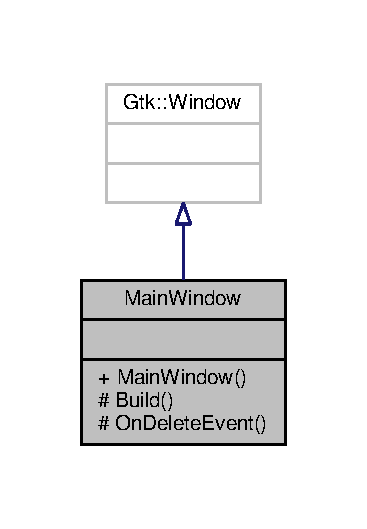
\includegraphics[width=176pt]{classMainWindow__inherit__graph}
\end{center}
\end{figure}


Collaboration diagram for Main\-Window\-:\nopagebreak
\begin{figure}[H]
\begin{center}
\leavevmode
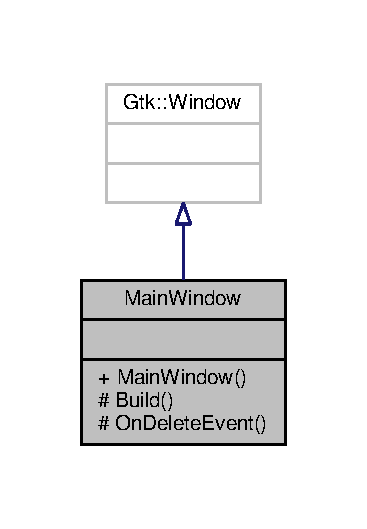
\includegraphics[width=176pt]{classMainWindow__coll__graph}
\end{center}
\end{figure}
\subsection*{Public Member Functions}
\begin{DoxyCompactItemize}
\item 
\hyperlink{classMainWindow_af607d50e4d1b04d3c494661489283f45}{Main\-Window} ()
\end{DoxyCompactItemize}
\subsection*{Protected Member Functions}
\begin{DoxyCompactItemize}
\item 
virtual void \hyperlink{classMainWindow_a952a77b964806830814cf4cdfbb2f0b9}{Build} ()
\item 
void \hyperlink{classMainWindow_a64bdcb29cebb58957790da1ee2733fe1}{On\-Delete\-Event} (object sender, Delete\-Event\-Args a)
\end{DoxyCompactItemize}


\subsection{Constructor \& Destructor Documentation}
\hypertarget{classMainWindow_af607d50e4d1b04d3c494661489283f45}{\index{Main\-Window@{Main\-Window}!Main\-Window@{Main\-Window}}
\index{Main\-Window@{Main\-Window}!MainWindow@{Main\-Window}}
\subsubsection[{Main\-Window}]{\setlength{\rightskip}{0pt plus 5cm}Main\-Window.\-Main\-Window (
\begin{DoxyParamCaption}
{}
\end{DoxyParamCaption}
)\hspace{0.3cm}{\ttfamily [inline]}}}\label{classMainWindow_af607d50e4d1b04d3c494661489283f45}


Here is the call graph for this function\-:\nopagebreak
\begin{figure}[H]
\begin{center}
\leavevmode
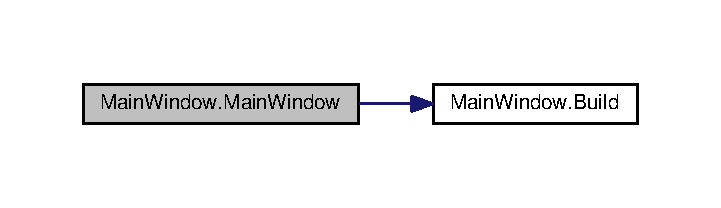
\includegraphics[width=346pt]{classMainWindow_af607d50e4d1b04d3c494661489283f45_cgraph}
\end{center}
\end{figure}




\subsection{Member Function Documentation}
\hypertarget{classMainWindow_a952a77b964806830814cf4cdfbb2f0b9}{\index{Main\-Window@{Main\-Window}!Build@{Build}}
\index{Build@{Build}!MainWindow@{Main\-Window}}
\subsubsection[{Build}]{\setlength{\rightskip}{0pt plus 5cm}virtual void Main\-Window.\-Build (
\begin{DoxyParamCaption}
{}
\end{DoxyParamCaption}
)\hspace{0.3cm}{\ttfamily [inline]}, {\ttfamily [protected]}, {\ttfamily [virtual]}}}\label{classMainWindow_a952a77b964806830814cf4cdfbb2f0b9}


Here is the caller graph for this function\-:\nopagebreak
\begin{figure}[H]
\begin{center}
\leavevmode
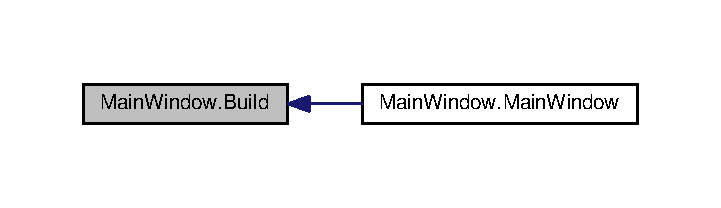
\includegraphics[width=346pt]{classMainWindow_a952a77b964806830814cf4cdfbb2f0b9_icgraph}
\end{center}
\end{figure}


\hypertarget{classMainWindow_a64bdcb29cebb58957790da1ee2733fe1}{\index{Main\-Window@{Main\-Window}!On\-Delete\-Event@{On\-Delete\-Event}}
\index{On\-Delete\-Event@{On\-Delete\-Event}!MainWindow@{Main\-Window}}
\subsubsection[{On\-Delete\-Event}]{\setlength{\rightskip}{0pt plus 5cm}void Main\-Window.\-On\-Delete\-Event (
\begin{DoxyParamCaption}
\item[{object}]{sender, }
\item[{Delete\-Event\-Args}]{a}
\end{DoxyParamCaption}
)\hspace{0.3cm}{\ttfamily [inline]}, {\ttfamily [protected]}}}\label{classMainWindow_a64bdcb29cebb58957790da1ee2733fe1}


The documentation for this class was generated from the following file\-:\begin{DoxyCompactItemize}
\item 
Net\-Traffic\-Simulator/\-Net\-Traffic\-Simulator/gtk-\/gui/\hyperlink{gtk-gui_2MainWindow_8cs}{Main\-Window.\-cs}\end{DoxyCompactItemize}

\hypertarget{classNetTrafficSimulator_1_1NetworkModel}{\section{Net\-Traffic\-Simulator.\-Network\-Model Class Reference}
\label{classNetTrafficSimulator_1_1NetworkModel}\index{Net\-Traffic\-Simulator.\-Network\-Model@{Net\-Traffic\-Simulator.\-Network\-Model}}
}
\subsection*{Public Member Functions}
\begin{DoxyCompactItemize}
\item 
\hyperlink{classNetTrafficSimulator_1_1NetworkModel_a271752106d40e56f0f55def7f0e1bf0d}{Network\-Model} (int \hyperlink{classNetTrafficSimulator_1_1NetworkModel_a85f9941bb3af088bd078b273f0cb4e52}{node\-\_\-count})
\item 
bool \hyperlink{classNetTrafficSimulator_1_1NetworkModel_a5d2d13396e4df9e45146b8a7f02a9b67}{Are\-Connected} (int x, int y)
\item 
void \hyperlink{classNetTrafficSimulator_1_1NetworkModel_a9b2e702172bb308e9882de6e1f22e9f1}{Set\-Connected} (int x, int y)
\item 
void \hyperlink{classNetTrafficSimulator_1_1NetworkModel_acf61bc6091630b26455868a2575d34c7}{Set\-Disconnected} (int x, int y)
\item 
int \hyperlink{classNetTrafficSimulator_1_1NetworkModel_ae32e3d246753b51152124af9df9372ee}{Get\-Connection\-Count} (int node)
\item 
int \hyperlink{classNetTrafficSimulator_1_1NetworkModel_a3d8f3112c2cc4b21fe8070a0896652fa}{Get\-Node\-Type} (int node)
\item 
void \hyperlink{classNetTrafficSimulator_1_1NetworkModel_ac8457d8aa77448caa2212020f48eec20}{Set\-Node\-Type} (int node, int type)
\item 
void \hyperlink{classNetTrafficSimulator_1_1NetworkModel_a724d036cf0dbadefaba005aa853630be}{Print} ()
\end{DoxyCompactItemize}
\subsection*{Public Attributes}
\begin{DoxyCompactItemize}
\item 
const int \hyperlink{classNetTrafficSimulator_1_1NetworkModel_a1335e5ee160345ac2f849998d94f2934}{E\-N\-D\-\_\-\-N\-O\-D\-E} = 0
\item 
const int \hyperlink{classNetTrafficSimulator_1_1NetworkModel_a9f536ecef65ce9ef55b52afa90ae8438}{S\-E\-R\-V\-E\-R\-\_\-\-N\-O\-D\-E} = 1
\item 
const int \hyperlink{classNetTrafficSimulator_1_1NetworkModel_ab2882fa4fe981780f78f822b12677f88}{N\-E\-T\-W\-O\-R\-K\-\_\-\-N\-O\-D\-E} = 2
\item 
const int \hyperlink{classNetTrafficSimulator_1_1NetworkModel_a6736303b5919398aef63238c6436fe9c}{U\-N\-I\-D\-E\-N\-T\-I\-F\-I\-E\-D\-\_\-\-N\-O\-D\-E} = -\/1
\end{DoxyCompactItemize}
\subsection*{Properties}
\begin{DoxyCompactItemize}
\item 
int \hyperlink{classNetTrafficSimulator_1_1NetworkModel_ae999583acaea839a7611f610bed2fed6}{Node\-Count}\hspace{0.3cm}{\ttfamily  \mbox{[}get\mbox{]}}
\item 
bool\mbox{[},\mbox{]} \hyperlink{classNetTrafficSimulator_1_1NetworkModel_aa1466fa74cbddeefb31b5d7369db983e}{Link}\hspace{0.3cm}{\ttfamily  \mbox{[}get\mbox{]}}
\item 
int\mbox{[}$\,$\mbox{]} \hyperlink{classNetTrafficSimulator_1_1NetworkModel_a92df1a7e9c05637930eae22d788f7c18}{Type}\hspace{0.3cm}{\ttfamily  \mbox{[}get\mbox{]}}
\item 
int\mbox{[}$\,$\mbox{]} \hyperlink{classNetTrafficSimulator_1_1NetworkModel_ad5eb61d192908f46907fd7f91f796691}{Link\-Count}\hspace{0.3cm}{\ttfamily  \mbox{[}get\mbox{]}}
\item 
bool \hyperlink{classNetTrafficSimulator_1_1NetworkModel_a58af85d9a9121926149ef5e2ce332e76}{Valid}\hspace{0.3cm}{\ttfamily  \mbox{[}get\mbox{]}}
\end{DoxyCompactItemize}
\subsection*{Private Attributes}
\begin{DoxyCompactItemize}
\item 
const string \hyperlink{classNetTrafficSimulator_1_1NetworkModel_a9ff3800009133089edb0744d2771b0b9}{I\-L\-L\-E\-G\-A\-L\-\_\-\-P\-A\-R\-A\-M\-E\-T\-E\-R} = \char`\"{}Neplatny parametr\char`\"{}
\item 
int \hyperlink{classNetTrafficSimulator_1_1NetworkModel_a85f9941bb3af088bd078b273f0cb4e52}{node\-\_\-count}
\item 
bool\mbox{[},\mbox{]} \hyperlink{classNetTrafficSimulator_1_1NetworkModel_a01410c5733a30fb4e37208c8b94fdf8d}{links}
\item 
int\mbox{[}$\,$\mbox{]} \hyperlink{classNetTrafficSimulator_1_1NetworkModel_a1437bfc2aad1a396054b03452e60c0dd}{link\-\_\-count}
\item 
int\mbox{[}$\,$\mbox{]} \hyperlink{classNetTrafficSimulator_1_1NetworkModel_aa8f0b62fb9e9029f0068135b56a46a9c}{types}
\end{DoxyCompactItemize}


\subsection{Detailed Description}
\hyperlink{classNetTrafficSimulator_1_1NetworkModel}{Network\-Model} generates network map based on data provided by user.

Network map is a graph represented as adjacency matrix.

Node can be of type E\-N\-D\-\_\-\-N\-O\-D\-E, S\-E\-R\-V\-E\-R\-\_\-\-N\-O\-D\-E, N\-E\-T\-W\-O\-R\-K\-\_\-\-N\-O\-D\-E or U\-N\-I\-D\-E\-N\-T\-I\-F\-I\-E\-D\-\_\-\-N\-O\-D\-E

\subsection{Constructor \& Destructor Documentation}
\hypertarget{classNetTrafficSimulator_1_1NetworkModel_a271752106d40e56f0f55def7f0e1bf0d}{\index{Net\-Traffic\-Simulator\-::\-Network\-Model@{Net\-Traffic\-Simulator\-::\-Network\-Model}!Network\-Model@{Network\-Model}}
\index{Network\-Model@{Network\-Model}!NetTrafficSimulator::NetworkModel@{Net\-Traffic\-Simulator\-::\-Network\-Model}}
\subsubsection[{Network\-Model}]{\setlength{\rightskip}{0pt plus 5cm}Net\-Traffic\-Simulator.\-Network\-Model.\-Network\-Model (
\begin{DoxyParamCaption}
\item[{int}]{node\-\_\-count}
\end{DoxyParamCaption}
)\hspace{0.3cm}{\ttfamily [inline]}}}\label{classNetTrafficSimulator_1_1NetworkModel_a271752106d40e56f0f55def7f0e1bf0d}
Creates a \hyperlink{classNetTrafficSimulator_1_1NetworkModel}{Network\-Model} with given amount of nodes 
\begin{DoxyParams}{Parameters}
{\em node\-\_\-count} & amount of nodes in model \\
\hline
\end{DoxyParams}

\begin{DoxyExceptions}{Exceptions}
{\em Argument\-Out\-Of\-Range\-Exception} & if given node\-\_\-count is less than 0 \\
\hline
\end{DoxyExceptions}


\subsection{Member Function Documentation}
\hypertarget{classNetTrafficSimulator_1_1NetworkModel_a5d2d13396e4df9e45146b8a7f02a9b67}{\index{Net\-Traffic\-Simulator\-::\-Network\-Model@{Net\-Traffic\-Simulator\-::\-Network\-Model}!Are\-Connected@{Are\-Connected}}
\index{Are\-Connected@{Are\-Connected}!NetTrafficSimulator::NetworkModel@{Net\-Traffic\-Simulator\-::\-Network\-Model}}
\subsubsection[{Are\-Connected}]{\setlength{\rightskip}{0pt plus 5cm}bool Net\-Traffic\-Simulator.\-Network\-Model.\-Are\-Connected (
\begin{DoxyParamCaption}
\item[{int}]{x, }
\item[{int}]{y}
\end{DoxyParamCaption}
)\hspace{0.3cm}{\ttfamily [inline]}}}\label{classNetTrafficSimulator_1_1NetworkModel_a5d2d13396e4df9e45146b8a7f02a9b67}
True if there is a direct link between nodes x and y 
\begin{DoxyParams}{Parameters}
{\em x} & node \\
\hline
{\em y} & node \\
\hline
\end{DoxyParams}
\begin{DoxyReturn}{Returns}
if there's a link 
\end{DoxyReturn}

\begin{DoxyExceptions}{Exceptions}
{\em Argument\-Out\-Of\-Range\-Exception} & when x or y are incorrect \\
\hline
\end{DoxyExceptions}
\hypertarget{classNetTrafficSimulator_1_1NetworkModel_ae32e3d246753b51152124af9df9372ee}{\index{Net\-Traffic\-Simulator\-::\-Network\-Model@{Net\-Traffic\-Simulator\-::\-Network\-Model}!Get\-Connection\-Count@{Get\-Connection\-Count}}
\index{Get\-Connection\-Count@{Get\-Connection\-Count}!NetTrafficSimulator::NetworkModel@{Net\-Traffic\-Simulator\-::\-Network\-Model}}
\subsubsection[{Get\-Connection\-Count}]{\setlength{\rightskip}{0pt plus 5cm}int Net\-Traffic\-Simulator.\-Network\-Model.\-Get\-Connection\-Count (
\begin{DoxyParamCaption}
\item[{int}]{node}
\end{DoxyParamCaption}
)\hspace{0.3cm}{\ttfamily [inline]}}}\label{classNetTrafficSimulator_1_1NetworkModel_ae32e3d246753b51152124af9df9372ee}
For given node returns value of link\-\_\-count counter 
\begin{DoxyParams}{Parameters}
{\em node} & node of interest \\
\hline
\end{DoxyParams}
\begin{DoxyReturn}{Returns}
amount of direct links connected to that node 
\end{DoxyReturn}

\begin{DoxyExceptions}{Exceptions}
{\em Argument\-Out\-Of\-Range\-Exception} & if node is incorrect \\
\hline
\end{DoxyExceptions}
\hypertarget{classNetTrafficSimulator_1_1NetworkModel_a3d8f3112c2cc4b21fe8070a0896652fa}{\index{Net\-Traffic\-Simulator\-::\-Network\-Model@{Net\-Traffic\-Simulator\-::\-Network\-Model}!Get\-Node\-Type@{Get\-Node\-Type}}
\index{Get\-Node\-Type@{Get\-Node\-Type}!NetTrafficSimulator::NetworkModel@{Net\-Traffic\-Simulator\-::\-Network\-Model}}
\subsubsection[{Get\-Node\-Type}]{\setlength{\rightskip}{0pt plus 5cm}int Net\-Traffic\-Simulator.\-Network\-Model.\-Get\-Node\-Type (
\begin{DoxyParamCaption}
\item[{int}]{node}
\end{DoxyParamCaption}
)\hspace{0.3cm}{\ttfamily [inline]}}}\label{classNetTrafficSimulator_1_1NetworkModel_a3d8f3112c2cc4b21fe8070a0896652fa}
For given node returns a type of node 
\begin{DoxyParams}{Parameters}
{\em node} & a node of interest \\
\hline
\end{DoxyParams}
\begin{DoxyReturn}{Returns}
one of following constants\-: E\-N\-D\-\_\-\-N\-O\-D\-E, S\-E\-R\-V\-E\-R\-\_\-\-N\-O\-D\-E, N\-E\-T\-W\-O\-R\-K\-\_\-\-N\-O\-D\-E, U\-N\-I\-D\-E\-N\-T\-I\-F\-I\-E\-D\-\_\-\-N\-O\-D\-E 
\end{DoxyReturn}

\begin{DoxyExceptions}{Exceptions}
{\em Argument\-Out\-Of\-Range\-Exception} & if given node is incorrect \\
\hline
\end{DoxyExceptions}
\hypertarget{classNetTrafficSimulator_1_1NetworkModel_a724d036cf0dbadefaba005aa853630be}{\index{Net\-Traffic\-Simulator\-::\-Network\-Model@{Net\-Traffic\-Simulator\-::\-Network\-Model}!Print@{Print}}
\index{Print@{Print}!NetTrafficSimulator::NetworkModel@{Net\-Traffic\-Simulator\-::\-Network\-Model}}
\subsubsection[{Print}]{\setlength{\rightskip}{0pt plus 5cm}void Net\-Traffic\-Simulator.\-Network\-Model.\-Print (
\begin{DoxyParamCaption}
{}
\end{DoxyParamCaption}
)\hspace{0.3cm}{\ttfamily [inline]}}}\label{classNetTrafficSimulator_1_1NetworkModel_a724d036cf0dbadefaba005aa853630be}
Prints matrix of adjacency and node type for each node on Console

E\-N\-D\-\_\-\-N\-O\-D\-E is marked as E\-N

S\-E\-R\-V\-E\-R\-\_\-\-N\-O\-D\-E is marked as S\-N

N\-E\-T\-W\-O\-R\-K\-\_\-\-N\-O\-D\-E is marked as N\-N

otherwise type is marked as N/\-A\hypertarget{classNetTrafficSimulator_1_1NetworkModel_a9b2e702172bb308e9882de6e1f22e9f1}{\index{Net\-Traffic\-Simulator\-::\-Network\-Model@{Net\-Traffic\-Simulator\-::\-Network\-Model}!Set\-Connected@{Set\-Connected}}
\index{Set\-Connected@{Set\-Connected}!NetTrafficSimulator::NetworkModel@{Net\-Traffic\-Simulator\-::\-Network\-Model}}
\subsubsection[{Set\-Connected}]{\setlength{\rightskip}{0pt plus 5cm}void Net\-Traffic\-Simulator.\-Network\-Model.\-Set\-Connected (
\begin{DoxyParamCaption}
\item[{int}]{x, }
\item[{int}]{y}
\end{DoxyParamCaption}
)\hspace{0.3cm}{\ttfamily [inline]}}}\label{classNetTrafficSimulator_1_1NetworkModel_a9b2e702172bb308e9882de6e1f22e9f1}
Marks a direct link between nodes x and y.

If there wasn't link yet, increments appropriate link\-\_\-count counters


\begin{DoxyParams}{Parameters}
{\em x} & node \\
\hline
{\em y} & node \\
\hline
\end{DoxyParams}

\begin{DoxyExceptions}{Exceptions}
{\em Argument\-Out\-Of\-Range\-Exception} & if x or y are incorrect \\
\hline
\end{DoxyExceptions}
\hypertarget{classNetTrafficSimulator_1_1NetworkModel_acf61bc6091630b26455868a2575d34c7}{\index{Net\-Traffic\-Simulator\-::\-Network\-Model@{Net\-Traffic\-Simulator\-::\-Network\-Model}!Set\-Disconnected@{Set\-Disconnected}}
\index{Set\-Disconnected@{Set\-Disconnected}!NetTrafficSimulator::NetworkModel@{Net\-Traffic\-Simulator\-::\-Network\-Model}}
\subsubsection[{Set\-Disconnected}]{\setlength{\rightskip}{0pt plus 5cm}void Net\-Traffic\-Simulator.\-Network\-Model.\-Set\-Disconnected (
\begin{DoxyParamCaption}
\item[{int}]{x, }
\item[{int}]{y}
\end{DoxyParamCaption}
)\hspace{0.3cm}{\ttfamily [inline]}}}\label{classNetTrafficSimulator_1_1NetworkModel_acf61bc6091630b26455868a2575d34c7}
Ensures there's no direct link between nodes x and y

If there previously was a direct link, also decrements link\-\_\-count counters


\begin{DoxyParams}{Parameters}
{\em x} & node \\
\hline
{\em y} & node \\
\hline
\end{DoxyParams}

\begin{DoxyExceptions}{Exceptions}
{\em Argument\-Out\-Of\-Range\-Exception} & if x or y are incorrect \\
\hline
\end{DoxyExceptions}
\hypertarget{classNetTrafficSimulator_1_1NetworkModel_ac8457d8aa77448caa2212020f48eec20}{\index{Net\-Traffic\-Simulator\-::\-Network\-Model@{Net\-Traffic\-Simulator\-::\-Network\-Model}!Set\-Node\-Type@{Set\-Node\-Type}}
\index{Set\-Node\-Type@{Set\-Node\-Type}!NetTrafficSimulator::NetworkModel@{Net\-Traffic\-Simulator\-::\-Network\-Model}}
\subsubsection[{Set\-Node\-Type}]{\setlength{\rightskip}{0pt plus 5cm}void Net\-Traffic\-Simulator.\-Network\-Model.\-Set\-Node\-Type (
\begin{DoxyParamCaption}
\item[{int}]{node, }
\item[{int}]{type}
\end{DoxyParamCaption}
)\hspace{0.3cm}{\ttfamily [inline]}}}\label{classNetTrafficSimulator_1_1NetworkModel_ac8457d8aa77448caa2212020f48eec20}
For given node sets a type of node 
\begin{DoxyParams}{Parameters}
{\em node} & a node of interest \\
\hline
{\em type} & one of following constants\-: E\-N\-D\-\_\-\-N\-O\-D\-E,S\-E\-R\-V\-E\-R\-\_\-\-N\-O\-D\-E,N\-E\-T\-W\-O\-R\-K\-\_\-\-N\-O\-D\-E \\
\hline
\end{DoxyParams}

\begin{DoxyExceptions}{Exceptions}
{\em Argument\-Out\-Of\-Range\-Exception} & if given node is incorrect or type is U\-N\-I\-D\-E\-N\-T\-I\-F\-I\-E\-D\-\_\-\-N\-O\-D\-E or is not any of declared constants \\
\hline
\end{DoxyExceptions}


\subsection{Member Data Documentation}
\hypertarget{classNetTrafficSimulator_1_1NetworkModel_a1335e5ee160345ac2f849998d94f2934}{\index{Net\-Traffic\-Simulator\-::\-Network\-Model@{Net\-Traffic\-Simulator\-::\-Network\-Model}!E\-N\-D\-\_\-\-N\-O\-D\-E@{E\-N\-D\-\_\-\-N\-O\-D\-E}}
\index{E\-N\-D\-\_\-\-N\-O\-D\-E@{E\-N\-D\-\_\-\-N\-O\-D\-E}!NetTrafficSimulator::NetworkModel@{Net\-Traffic\-Simulator\-::\-Network\-Model}}
\subsubsection[{E\-N\-D\-\_\-\-N\-O\-D\-E}]{\setlength{\rightskip}{0pt plus 5cm}const int Net\-Traffic\-Simulator.\-Network\-Model.\-E\-N\-D\-\_\-\-N\-O\-D\-E = 0}}\label{classNetTrafficSimulator_1_1NetworkModel_a1335e5ee160345ac2f849998d94f2934}
E\-N\-D\-\_\-\-N\-O\-D\-E is a end-\/user node, which initiates connection to server-\/node \hypertarget{classNetTrafficSimulator_1_1NetworkModel_a9ff3800009133089edb0744d2771b0b9}{\index{Net\-Traffic\-Simulator\-::\-Network\-Model@{Net\-Traffic\-Simulator\-::\-Network\-Model}!I\-L\-L\-E\-G\-A\-L\-\_\-\-P\-A\-R\-A\-M\-E\-T\-E\-R@{I\-L\-L\-E\-G\-A\-L\-\_\-\-P\-A\-R\-A\-M\-E\-T\-E\-R}}
\index{I\-L\-L\-E\-G\-A\-L\-\_\-\-P\-A\-R\-A\-M\-E\-T\-E\-R@{I\-L\-L\-E\-G\-A\-L\-\_\-\-P\-A\-R\-A\-M\-E\-T\-E\-R}!NetTrafficSimulator::NetworkModel@{Net\-Traffic\-Simulator\-::\-Network\-Model}}
\subsubsection[{I\-L\-L\-E\-G\-A\-L\-\_\-\-P\-A\-R\-A\-M\-E\-T\-E\-R}]{\setlength{\rightskip}{0pt plus 5cm}const string Net\-Traffic\-Simulator.\-Network\-Model.\-I\-L\-L\-E\-G\-A\-L\-\_\-\-P\-A\-R\-A\-M\-E\-T\-E\-R = \char`\"{}Neplatny parametr\char`\"{}\hspace{0.3cm}{\ttfamily [private]}}}\label{classNetTrafficSimulator_1_1NetworkModel_a9ff3800009133089edb0744d2771b0b9}
Message string added to any illegal argument exception thrown \hypertarget{classNetTrafficSimulator_1_1NetworkModel_a1437bfc2aad1a396054b03452e60c0dd}{\index{Net\-Traffic\-Simulator\-::\-Network\-Model@{Net\-Traffic\-Simulator\-::\-Network\-Model}!link\-\_\-count@{link\-\_\-count}}
\index{link\-\_\-count@{link\-\_\-count}!NetTrafficSimulator::NetworkModel@{Net\-Traffic\-Simulator\-::\-Network\-Model}}
\subsubsection[{link\-\_\-count}]{\setlength{\rightskip}{0pt plus 5cm}int \mbox{[}$\,$\mbox{]} Net\-Traffic\-Simulator.\-Network\-Model.\-link\-\_\-count\hspace{0.3cm}{\ttfamily [private]}}}\label{classNetTrafficSimulator_1_1NetworkModel_a1437bfc2aad1a396054b03452e60c0dd}
link\-\_\-count\mbox{[}x\mbox{]} is amount of links connected to a node x \hypertarget{classNetTrafficSimulator_1_1NetworkModel_a01410c5733a30fb4e37208c8b94fdf8d}{\index{Net\-Traffic\-Simulator\-::\-Network\-Model@{Net\-Traffic\-Simulator\-::\-Network\-Model}!links@{links}}
\index{links@{links}!NetTrafficSimulator::NetworkModel@{Net\-Traffic\-Simulator\-::\-Network\-Model}}
\subsubsection[{links}]{\setlength{\rightskip}{0pt plus 5cm}bool \mbox{[},\mbox{]} Net\-Traffic\-Simulator.\-Network\-Model.\-links\hspace{0.3cm}{\ttfamily [private]}}}\label{classNetTrafficSimulator_1_1NetworkModel_a01410c5733a30fb4e37208c8b94fdf8d}
Adjacency matrix of the network\-: links\mbox{[}x,y\mbox{]} is true if there is a direct connection between nodes x and y \hypertarget{classNetTrafficSimulator_1_1NetworkModel_ab2882fa4fe981780f78f822b12677f88}{\index{Net\-Traffic\-Simulator\-::\-Network\-Model@{Net\-Traffic\-Simulator\-::\-Network\-Model}!N\-E\-T\-W\-O\-R\-K\-\_\-\-N\-O\-D\-E@{N\-E\-T\-W\-O\-R\-K\-\_\-\-N\-O\-D\-E}}
\index{N\-E\-T\-W\-O\-R\-K\-\_\-\-N\-O\-D\-E@{N\-E\-T\-W\-O\-R\-K\-\_\-\-N\-O\-D\-E}!NetTrafficSimulator::NetworkModel@{Net\-Traffic\-Simulator\-::\-Network\-Model}}
\subsubsection[{N\-E\-T\-W\-O\-R\-K\-\_\-\-N\-O\-D\-E}]{\setlength{\rightskip}{0pt plus 5cm}const int Net\-Traffic\-Simulator.\-Network\-Model.\-N\-E\-T\-W\-O\-R\-K\-\_\-\-N\-O\-D\-E = 2}}\label{classNetTrafficSimulator_1_1NetworkModel_ab2882fa4fe981780f78f822b12677f88}
N\-E\-T\-W\-O\-R\-K\-\_\-\-N\-O\-D\-E is router / switch on the network \hypertarget{classNetTrafficSimulator_1_1NetworkModel_a85f9941bb3af088bd078b273f0cb4e52}{\index{Net\-Traffic\-Simulator\-::\-Network\-Model@{Net\-Traffic\-Simulator\-::\-Network\-Model}!node\-\_\-count@{node\-\_\-count}}
\index{node\-\_\-count@{node\-\_\-count}!NetTrafficSimulator::NetworkModel@{Net\-Traffic\-Simulator\-::\-Network\-Model}}
\subsubsection[{node\-\_\-count}]{\setlength{\rightskip}{0pt plus 5cm}int Net\-Traffic\-Simulator.\-Network\-Model.\-node\-\_\-count\hspace{0.3cm}{\ttfamily [private]}}}\label{classNetTrafficSimulator_1_1NetworkModel_a85f9941bb3af088bd078b273f0cb4e52}
Amount of nodes in the model \hypertarget{classNetTrafficSimulator_1_1NetworkModel_a9f536ecef65ce9ef55b52afa90ae8438}{\index{Net\-Traffic\-Simulator\-::\-Network\-Model@{Net\-Traffic\-Simulator\-::\-Network\-Model}!S\-E\-R\-V\-E\-R\-\_\-\-N\-O\-D\-E@{S\-E\-R\-V\-E\-R\-\_\-\-N\-O\-D\-E}}
\index{S\-E\-R\-V\-E\-R\-\_\-\-N\-O\-D\-E@{S\-E\-R\-V\-E\-R\-\_\-\-N\-O\-D\-E}!NetTrafficSimulator::NetworkModel@{Net\-Traffic\-Simulator\-::\-Network\-Model}}
\subsubsection[{S\-E\-R\-V\-E\-R\-\_\-\-N\-O\-D\-E}]{\setlength{\rightskip}{0pt plus 5cm}const int Net\-Traffic\-Simulator.\-Network\-Model.\-S\-E\-R\-V\-E\-R\-\_\-\-N\-O\-D\-E = 1}}\label{classNetTrafficSimulator_1_1NetworkModel_a9f536ecef65ce9ef55b52afa90ae8438}
S\-E\-R\-V\-E\-R\-\_\-\-N\-O\-D\-E is server, which responds to received packets \hypertarget{classNetTrafficSimulator_1_1NetworkModel_aa8f0b62fb9e9029f0068135b56a46a9c}{\index{Net\-Traffic\-Simulator\-::\-Network\-Model@{Net\-Traffic\-Simulator\-::\-Network\-Model}!types@{types}}
\index{types@{types}!NetTrafficSimulator::NetworkModel@{Net\-Traffic\-Simulator\-::\-Network\-Model}}
\subsubsection[{types}]{\setlength{\rightskip}{0pt plus 5cm}int \mbox{[}$\,$\mbox{]} Net\-Traffic\-Simulator.\-Network\-Model.\-types\hspace{0.3cm}{\ttfamily [private]}}}\label{classNetTrafficSimulator_1_1NetworkModel_aa8f0b62fb9e9029f0068135b56a46a9c}
types\mbox{[}x\mbox{]} is type of a node x \hypertarget{classNetTrafficSimulator_1_1NetworkModel_a6736303b5919398aef63238c6436fe9c}{\index{Net\-Traffic\-Simulator\-::\-Network\-Model@{Net\-Traffic\-Simulator\-::\-Network\-Model}!U\-N\-I\-D\-E\-N\-T\-I\-F\-I\-E\-D\-\_\-\-N\-O\-D\-E@{U\-N\-I\-D\-E\-N\-T\-I\-F\-I\-E\-D\-\_\-\-N\-O\-D\-E}}
\index{U\-N\-I\-D\-E\-N\-T\-I\-F\-I\-E\-D\-\_\-\-N\-O\-D\-E@{U\-N\-I\-D\-E\-N\-T\-I\-F\-I\-E\-D\-\_\-\-N\-O\-D\-E}!NetTrafficSimulator::NetworkModel@{Net\-Traffic\-Simulator\-::\-Network\-Model}}
\subsubsection[{U\-N\-I\-D\-E\-N\-T\-I\-F\-I\-E\-D\-\_\-\-N\-O\-D\-E}]{\setlength{\rightskip}{0pt plus 5cm}const int Net\-Traffic\-Simulator.\-Network\-Model.\-U\-N\-I\-D\-E\-N\-T\-I\-F\-I\-E\-D\-\_\-\-N\-O\-D\-E = -\/1}}\label{classNetTrafficSimulator_1_1NetworkModel_a6736303b5919398aef63238c6436fe9c}
U\-N\-I\-D\-E\-N\-T\-I\-F\-I\-E\-D\-\_\-\-N\-O\-D\-E indicates an error in model 

\subsection{Property Documentation}
\hypertarget{classNetTrafficSimulator_1_1NetworkModel_aa1466fa74cbddeefb31b5d7369db983e}{\index{Net\-Traffic\-Simulator\-::\-Network\-Model@{Net\-Traffic\-Simulator\-::\-Network\-Model}!Link@{Link}}
\index{Link@{Link}!NetTrafficSimulator::NetworkModel@{Net\-Traffic\-Simulator\-::\-Network\-Model}}
\subsubsection[{Link}]{\setlength{\rightskip}{0pt plus 5cm}bool \mbox{[},\mbox{]} Net\-Traffic\-Simulator.\-Network\-Model.\-Link\hspace{0.3cm}{\ttfamily [get]}}}\label{classNetTrafficSimulator_1_1NetworkModel_aa1466fa74cbddeefb31b5d7369db983e}
Adjacency matrix for the network \hypertarget{classNetTrafficSimulator_1_1NetworkModel_ad5eb61d192908f46907fd7f91f796691}{\index{Net\-Traffic\-Simulator\-::\-Network\-Model@{Net\-Traffic\-Simulator\-::\-Network\-Model}!Link\-Count@{Link\-Count}}
\index{Link\-Count@{Link\-Count}!NetTrafficSimulator::NetworkModel@{Net\-Traffic\-Simulator\-::\-Network\-Model}}
\subsubsection[{Link\-Count}]{\setlength{\rightskip}{0pt plus 5cm}int \mbox{[}$\,$\mbox{]} Net\-Traffic\-Simulator.\-Network\-Model.\-Link\-Count\hspace{0.3cm}{\ttfamily [get]}}}\label{classNetTrafficSimulator_1_1NetworkModel_ad5eb61d192908f46907fd7f91f796691}
Amount of links connected to nodes \hypertarget{classNetTrafficSimulator_1_1NetworkModel_ae999583acaea839a7611f610bed2fed6}{\index{Net\-Traffic\-Simulator\-::\-Network\-Model@{Net\-Traffic\-Simulator\-::\-Network\-Model}!Node\-Count@{Node\-Count}}
\index{Node\-Count@{Node\-Count}!NetTrafficSimulator::NetworkModel@{Net\-Traffic\-Simulator\-::\-Network\-Model}}
\subsubsection[{Node\-Count}]{\setlength{\rightskip}{0pt plus 5cm}int Net\-Traffic\-Simulator.\-Network\-Model.\-Node\-Count\hspace{0.3cm}{\ttfamily [get]}}}\label{classNetTrafficSimulator_1_1NetworkModel_ae999583acaea839a7611f610bed2fed6}
Amount of nodes in the model \hypertarget{classNetTrafficSimulator_1_1NetworkModel_a92df1a7e9c05637930eae22d788f7c18}{\index{Net\-Traffic\-Simulator\-::\-Network\-Model@{Net\-Traffic\-Simulator\-::\-Network\-Model}!Type@{Type}}
\index{Type@{Type}!NetTrafficSimulator::NetworkModel@{Net\-Traffic\-Simulator\-::\-Network\-Model}}
\subsubsection[{Type}]{\setlength{\rightskip}{0pt plus 5cm}int \mbox{[}$\,$\mbox{]} Net\-Traffic\-Simulator.\-Network\-Model.\-Type\hspace{0.3cm}{\ttfamily [get]}}}\label{classNetTrafficSimulator_1_1NetworkModel_a92df1a7e9c05637930eae22d788f7c18}
Types of nodes \hypertarget{classNetTrafficSimulator_1_1NetworkModel_a58af85d9a9121926149ef5e2ce332e76}{\index{Net\-Traffic\-Simulator\-::\-Network\-Model@{Net\-Traffic\-Simulator\-::\-Network\-Model}!Valid@{Valid}}
\index{Valid@{Valid}!NetTrafficSimulator::NetworkModel@{Net\-Traffic\-Simulator\-::\-Network\-Model}}
\subsubsection[{Valid}]{\setlength{\rightskip}{0pt plus 5cm}bool Net\-Traffic\-Simulator.\-Network\-Model.\-Valid\hspace{0.3cm}{\ttfamily [get]}}}\label{classNetTrafficSimulator_1_1NetworkModel_a58af85d9a9121926149ef5e2ce332e76}
Validates the model Model is valid if all following constraints are met\-:
\begin{DoxyItemize}
\item link count for each node is greater or equal to zero
\item link count for each node is less than amount of nodes in model
\item no node is connected to itself
\item only if node is N\-E\-T\-W\-O\-R\-K\-\_\-\-N\-O\-D\-E, it's link count is greater than 1
\item no node in model is U\-N\-I\-D\-E\-N\-T\-I\-F\-I\-E\-D\-\_\-\-N\-O\-D\-E
\item adjacency matrix is symmetric \begin{DoxyReturn}{Returns}
if model is valid or not 
\end{DoxyReturn}

\end{DoxyItemize}

The documentation for this class was generated from the following file\-:\begin{DoxyCompactItemize}
\item 
Net\-Traffic\-Simulator/\-Net\-Traffic\-Simulator/model/\hyperlink{NetworkModel_8cs}{Network\-Model.\-cs}\end{DoxyCompactItemize}

\hypertarget{classNetTrafficSimulator_1_1NetworkModelTest}{\section{Net\-Traffic\-Simulator.\-Network\-Model\-Test Class Reference}
\label{classNetTrafficSimulator_1_1NetworkModelTest}\index{Net\-Traffic\-Simulator.\-Network\-Model\-Test@{Net\-Traffic\-Simulator.\-Network\-Model\-Test}}
}


Collaboration diagram for Net\-Traffic\-Simulator.\-Network\-Model\-Test\-:\nopagebreak
\begin{figure}[H]
\begin{center}
\leavevmode
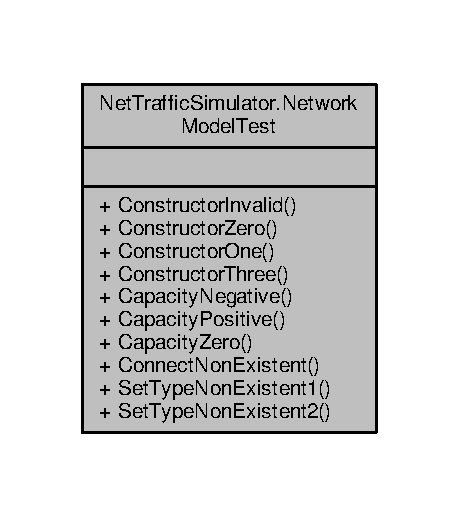
\includegraphics[width=220pt]{classNetTrafficSimulator_1_1NetworkModelTest__coll__graph}
\end{center}
\end{figure}
\subsection*{Public Member Functions}
\begin{DoxyCompactItemize}
\item 
void \hyperlink{classNetTrafficSimulator_1_1NetworkModelTest_afbd7470eb35b97512aa94a2f53163430}{Constructor\-Invalid} ()
\item 
void \hyperlink{classNetTrafficSimulator_1_1NetworkModelTest_a3634f2a5d0e008e7cd8b274615b173ee}{Constructor\-Zero} ()
\item 
void \hyperlink{classNetTrafficSimulator_1_1NetworkModelTest_a6a13d32fefa5e53b7f18e89b2fb8b436}{Constructor\-One} ()
\item 
void \hyperlink{classNetTrafficSimulator_1_1NetworkModelTest_a149aa9eab4b53fb17aa19be215e769b5}{Constructor\-Three} ()
\end{DoxyCompactItemize}


\subsection{Detailed Description}
Test of \hyperlink{classNetTrafficSimulator_1_1NetworkModel}{Network\-Model} class 

\subsection{Member Function Documentation}
\hypertarget{classNetTrafficSimulator_1_1NetworkModelTest_afbd7470eb35b97512aa94a2f53163430}{\index{Net\-Traffic\-Simulator\-::\-Network\-Model\-Test@{Net\-Traffic\-Simulator\-::\-Network\-Model\-Test}!Constructor\-Invalid@{Constructor\-Invalid}}
\index{Constructor\-Invalid@{Constructor\-Invalid}!NetTrafficSimulator::NetworkModelTest@{Net\-Traffic\-Simulator\-::\-Network\-Model\-Test}}
\subsubsection[{Constructor\-Invalid}]{\setlength{\rightskip}{0pt plus 5cm}void Net\-Traffic\-Simulator.\-Network\-Model\-Test.\-Constructor\-Invalid (
\begin{DoxyParamCaption}
{}
\end{DoxyParamCaption}
)\hspace{0.3cm}{\ttfamily [inline]}}}\label{classNetTrafficSimulator_1_1NetworkModelTest_afbd7470eb35b97512aa94a2f53163430}
Try to create model with -\/1 nodes \hypertarget{classNetTrafficSimulator_1_1NetworkModelTest_a6a13d32fefa5e53b7f18e89b2fb8b436}{\index{Net\-Traffic\-Simulator\-::\-Network\-Model\-Test@{Net\-Traffic\-Simulator\-::\-Network\-Model\-Test}!Constructor\-One@{Constructor\-One}}
\index{Constructor\-One@{Constructor\-One}!NetTrafficSimulator::NetworkModelTest@{Net\-Traffic\-Simulator\-::\-Network\-Model\-Test}}
\subsubsection[{Constructor\-One}]{\setlength{\rightskip}{0pt plus 5cm}void Net\-Traffic\-Simulator.\-Network\-Model\-Test.\-Constructor\-One (
\begin{DoxyParamCaption}
{}
\end{DoxyParamCaption}
)\hspace{0.3cm}{\ttfamily [inline]}}}\label{classNetTrafficSimulator_1_1NetworkModelTest_a6a13d32fefa5e53b7f18e89b2fb8b436}
Create model with one node. Assert node is initially unidentified and model invalid, assert node count and connection count. Set node to E\-N\-D\-\_\-\-N\-O\-D\-E type, verify Get\-Node\-Type and Type\mbox{[}0\mbox{]}. Assert model is valid. Print model onto Console. Assert link count. Assert no loop connection \mbox{[}0,0\mbox{]}. Create connection \mbox{[}0,0\mbox{]} and assert model is invalid. Print model onto Console. \hypertarget{classNetTrafficSimulator_1_1NetworkModelTest_a149aa9eab4b53fb17aa19be215e769b5}{\index{Net\-Traffic\-Simulator\-::\-Network\-Model\-Test@{Net\-Traffic\-Simulator\-::\-Network\-Model\-Test}!Constructor\-Three@{Constructor\-Three}}
\index{Constructor\-Three@{Constructor\-Three}!NetTrafficSimulator::NetworkModelTest@{Net\-Traffic\-Simulator\-::\-Network\-Model\-Test}}
\subsubsection[{Constructor\-Three}]{\setlength{\rightskip}{0pt plus 5cm}void Net\-Traffic\-Simulator.\-Network\-Model\-Test.\-Constructor\-Three (
\begin{DoxyParamCaption}
{}
\end{DoxyParamCaption}
)\hspace{0.3cm}{\ttfamily [inline]}}}\label{classNetTrafficSimulator_1_1NetworkModelTest_a149aa9eab4b53fb17aa19be215e769b5}
Create model with 3 elements. Assert all of them are unidentified and model is invalid. Assert node count and all connection counts. Set node types and assert validity. Create connections, print onto Console, assert validity, create invalid connection -\/ assert model not valid, fix and create different invalid connection, assert model not valid \hypertarget{classNetTrafficSimulator_1_1NetworkModelTest_a3634f2a5d0e008e7cd8b274615b173ee}{\index{Net\-Traffic\-Simulator\-::\-Network\-Model\-Test@{Net\-Traffic\-Simulator\-::\-Network\-Model\-Test}!Constructor\-Zero@{Constructor\-Zero}}
\index{Constructor\-Zero@{Constructor\-Zero}!NetTrafficSimulator::NetworkModelTest@{Net\-Traffic\-Simulator\-::\-Network\-Model\-Test}}
\subsubsection[{Constructor\-Zero}]{\setlength{\rightskip}{0pt plus 5cm}void Net\-Traffic\-Simulator.\-Network\-Model\-Test.\-Constructor\-Zero (
\begin{DoxyParamCaption}
{}
\end{DoxyParamCaption}
)\hspace{0.3cm}{\ttfamily [inline]}}}\label{classNetTrafficSimulator_1_1NetworkModelTest_a3634f2a5d0e008e7cd8b274615b173ee}
Create constructor with 0 nodes. Assert node count and validity 

The documentation for this class was generated from the following file\-:\begin{DoxyCompactItemize}
\item 
Net\-Traffic\-Simulator/\-Net\-Traffic\-Simulator/model/\hyperlink{NetworkModelTest_8cs}{Network\-Model\-Test.\-cs}\end{DoxyCompactItemize}

\chapter{File Documentation}
\hypertarget{generated_8cs}{\section{Net\-Traffic\-Simulator/\-Net\-Traffic\-Simulator/gtk-\/gui/generated.cs File Reference}
\label{generated_8cs}\index{Net\-Traffic\-Simulator/\-Net\-Traffic\-Simulator/gtk-\/gui/generated.\-cs@{Net\-Traffic\-Simulator/\-Net\-Traffic\-Simulator/gtk-\/gui/generated.\-cs}}
}
\subsection*{Classes}
\begin{DoxyCompactItemize}
\item 
class {\bfseries Stetic.\-Gui}
\item 
class {\bfseries Stetic.\-Action\-Groups}
\end{DoxyCompactItemize}
\subsection*{Namespaces}
\begin{DoxyCompactItemize}
\item 
package \hyperlink{namespaceStetic}{Stetic}
\end{DoxyCompactItemize}

\hypertarget{gtk-gui_2MainWindow_8cs}{\section{Net\-Traffic\-Simulator/\-Net\-Traffic\-Simulator/gtk-\/gui/\-Main\-Window.cs File Reference}
\label{gtk-gui_2MainWindow_8cs}\index{Net\-Traffic\-Simulator/\-Net\-Traffic\-Simulator/gtk-\/gui/\-Main\-Window.\-cs@{Net\-Traffic\-Simulator/\-Net\-Traffic\-Simulator/gtk-\/gui/\-Main\-Window.\-cs}}
}
\subsection*{Classes}
\begin{DoxyCompactItemize}
\item 
class \hyperlink{classMainWindow}{Main\-Window}
\end{DoxyCompactItemize}

\hypertarget{MainWindow_8cs}{\section{Net\-Traffic\-Simulator/\-Net\-Traffic\-Simulator/\-Main\-Window.cs File Reference}
\label{MainWindow_8cs}\index{Net\-Traffic\-Simulator/\-Net\-Traffic\-Simulator/\-Main\-Window.\-cs@{Net\-Traffic\-Simulator/\-Net\-Traffic\-Simulator/\-Main\-Window.\-cs}}
}
\subsection*{Classes}
\begin{DoxyCompactItemize}
\item 
class \hyperlink{classMainWindow}{Main\-Window}
\end{DoxyCompactItemize}

\hypertarget{NetworkModel_8cs}{\section{Net\-Traffic\-Simulator/\-Net\-Traffic\-Simulator/model/\-Network\-Model.cs File Reference}
\label{NetworkModel_8cs}\index{Net\-Traffic\-Simulator/\-Net\-Traffic\-Simulator/model/\-Network\-Model.\-cs@{Net\-Traffic\-Simulator/\-Net\-Traffic\-Simulator/model/\-Network\-Model.\-cs}}
}
\subsection*{Classes}
\begin{DoxyCompactItemize}
\item 
class \hyperlink{classNetTrafficSimulator_1_1NetworkModel}{Net\-Traffic\-Simulator.\-Network\-Model}
\end{DoxyCompactItemize}
\subsection*{Namespaces}
\begin{DoxyCompactItemize}
\item 
package \hyperlink{namespaceNetTrafficSimulator}{Net\-Traffic\-Simulator}
\end{DoxyCompactItemize}

\hypertarget{NetworkModelTest_8cs}{\section{Net\-Traffic\-Simulator/\-Net\-Traffic\-Simulator/model/\-Network\-Model\-Test.cs File Reference}
\label{NetworkModelTest_8cs}\index{Net\-Traffic\-Simulator/\-Net\-Traffic\-Simulator/model/\-Network\-Model\-Test.\-cs@{Net\-Traffic\-Simulator/\-Net\-Traffic\-Simulator/model/\-Network\-Model\-Test.\-cs}}
}
\subsection*{Classes}
\begin{DoxyCompactItemize}
\item 
class \hyperlink{classNetTrafficSimulator_1_1NetworkModelTest}{Net\-Traffic\-Simulator.\-Network\-Model\-Test}
\end{DoxyCompactItemize}
\subsection*{Namespaces}
\begin{DoxyCompactItemize}
\item 
package \hyperlink{namespaceNetTrafficSimulator}{Net\-Traffic\-Simulator}
\end{DoxyCompactItemize}

\hypertarget{Program_8cs}{\section{Net\-Traffic\-Simulator/\-Net\-Traffic\-Simulator/\-Program.cs File Reference}
\label{Program_8cs}\index{Net\-Traffic\-Simulator/\-Net\-Traffic\-Simulator/\-Program.\-cs@{Net\-Traffic\-Simulator/\-Net\-Traffic\-Simulator/\-Program.\-cs}}
}
\subsection*{Classes}
\begin{DoxyCompactItemize}
\item 
class \hyperlink{classNetTrafficSimulator_1_1MainClass}{Net\-Traffic\-Simulator.\-Main\-Class}
\end{DoxyCompactItemize}
\subsection*{Namespaces}
\begin{DoxyCompactItemize}
\item 
package \hyperlink{namespaceNetTrafficSimulator}{Net\-Traffic\-Simulator}
\end{DoxyCompactItemize}

\hypertarget{AssemblyInfo_8cs}{\section{Net\-Traffic\-Simulator/\-Net\-Traffic\-Simulator/\-Properties/\-Assembly\-Info.cs File Reference}
\label{AssemblyInfo_8cs}\index{Net\-Traffic\-Simulator/\-Net\-Traffic\-Simulator/\-Properties/\-Assembly\-Info.\-cs@{Net\-Traffic\-Simulator/\-Net\-Traffic\-Simulator/\-Properties/\-Assembly\-Info.\-cs}}
}

%--- End generated contents ---

% Index
\newpage
\phantomsection
\addcontentsline{toc}{chapter}{Index}
\printindex

\end{document}
